\section{Aggregation Methods: A Closer Look~\label{sec:agg-detailed}}
%Describe Tile based models. Briefly describe construction of tiles from BBs.
% In this section we formalize the problem of picking an optimal set of tiles, and describe our solution to this problem.
% \subsection{Definitions}
The key insight of aggregation-based methods is that they perform inference at a more fine-grained ``tile'' level, rather than at the bounding box level as is in the case of retrieval-based methods. In this section, we discuss three different algorithms for choosing a ``good'' set of worker tiles in aggregation-based methods.
%In this section, we discuss aggregation based methods which use combine the segmentations from multiple workers and output a single merged segmentation. As described earlier in Section~\ref{sec:crowd}, our aggregation algorithms first transform the set of worker segmentations into tiles, as shown in Fig.~\ref{tile_demo}, and then choose a set of tiles to include in the final segmentation. \todo[inline]{modify figure, or use from prev section if added.} Since aggregation based approaches work at the level of tiles, they are more fine-grained than retrieval-based methods, which work at the granularity of complete worker segmentations.
\begin{figure}
\centering
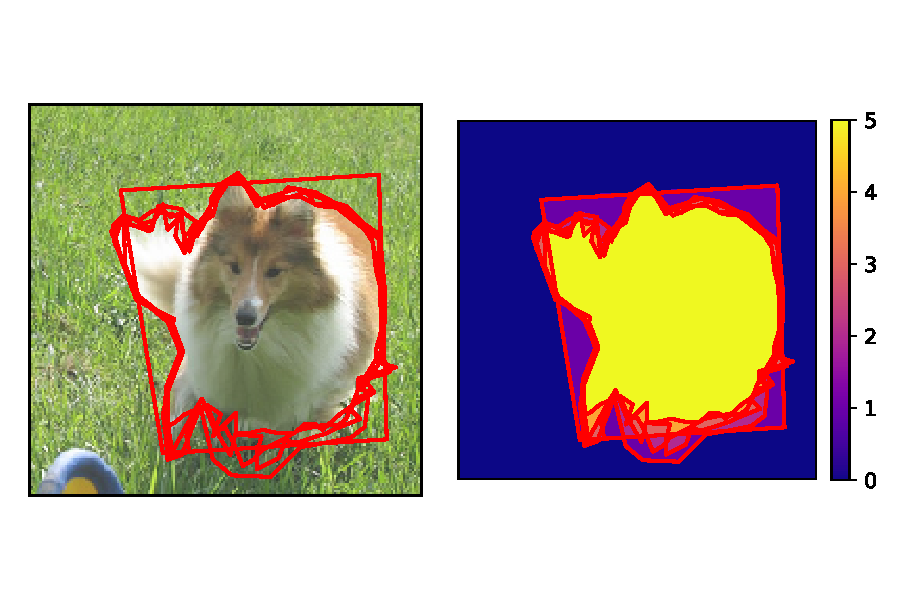
\includegraphics[width=\textwidth]{plots/tile_demo.pdf}
\caption{Left: Red boundaries shows the segmentation boundaries drawn by five workers overlaid on the image. Right: Segmentation boundaries still shown in red. The overlaid segmentation creates a masks where the color indicates the number of workers who voted for the tile region.}
\label{tile_demo}
\end{figure}
% \begin{figure}
% \centering
% 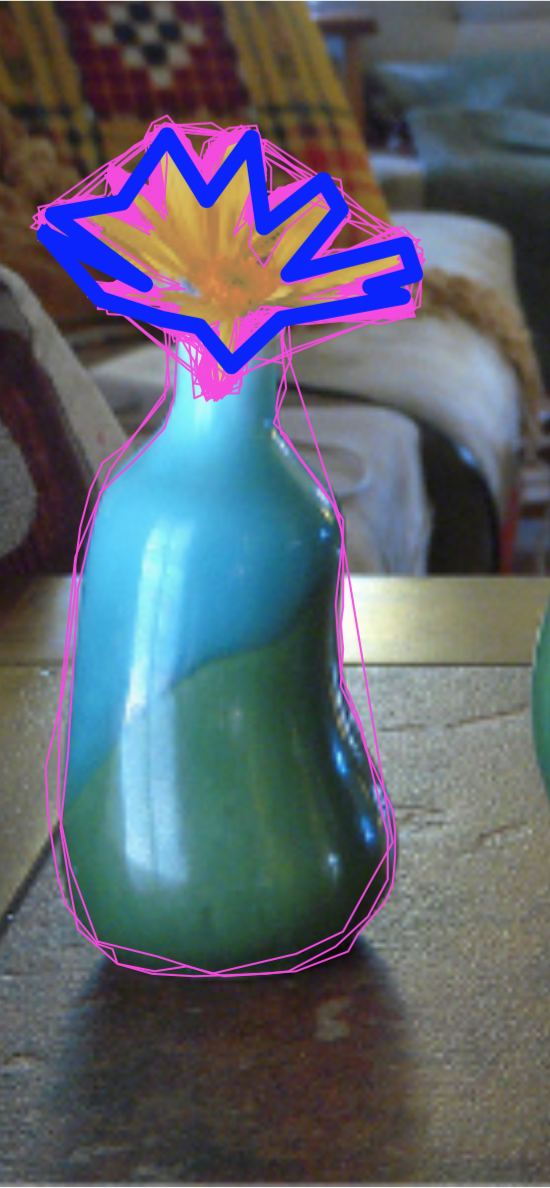
\includegraphics[width=.25\textwidth]{plots/worker_cropped.png}
% 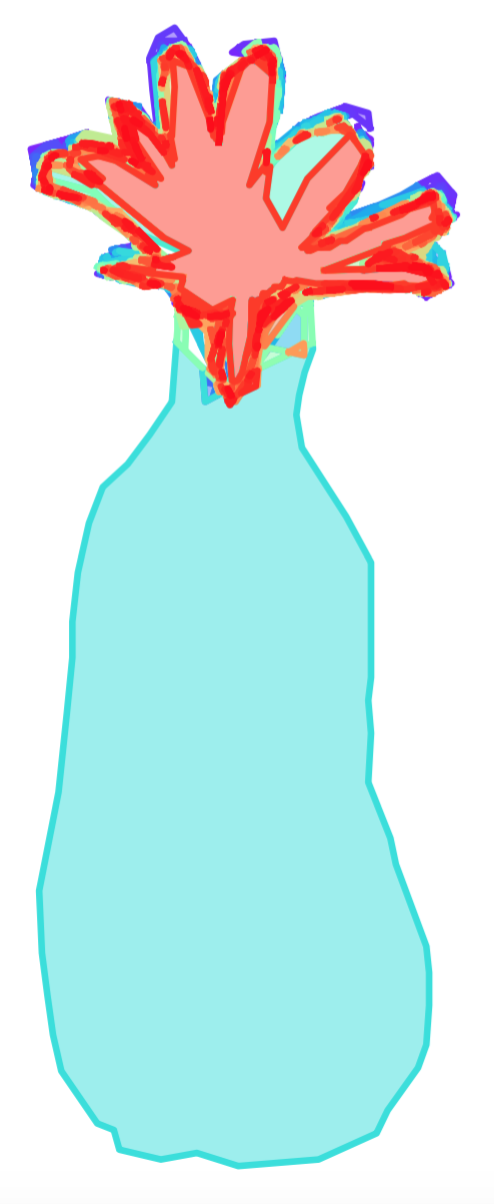
\includegraphics[width=.2\textwidth]{plots/tile_cropped.png}
% 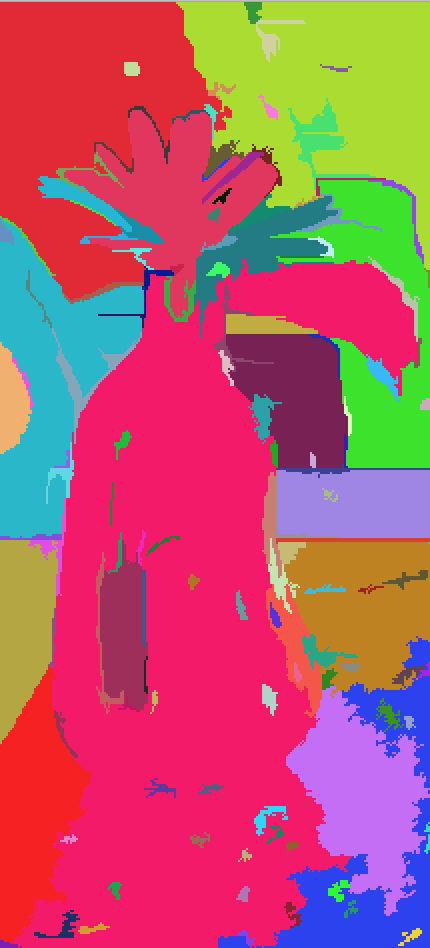
\includegraphics[width=.25\textwidth]{plots/vision_cropped.png}
% \caption{Left: Pink shows 40 worker bounding boxes for the object ``flower'' and blue ground truth segmentation, superimposed on the original COCO image. Center: Non-overlapping tiles constructed from worker bounding box. Right: Output from the color-segmentation vision algorithm.}
% \label{flower_example}
% \todo[inline]{Add black and white, vision segmented region image}
% \end{figure}
%Clarify that our search space is tile combination formed by all the worker's tiles not the space of all possible coordinates. (i.e. we assume that a region can not be inside the BB if no workers bounded that region)

\subsection{Majority Vote Aggregation (MV)}
A common strategy for aggregating multiple worker responses in crowdsourced algorithms is {\em Majority Vote}(MV)\dor{Akash: add citation for MV from general crowdsourcing domain}. In the context of choosing worker tiles to produce a segmentation, the natural Majority Vote algorithm looks at each tile, and includes the tile in the output segmentation if and only if the tile is covered by at least 50\% of all worker segmentations.
% We investigated three types of variants for majority vote strategies: picking the top-k, top-percentile tiles of vote counts and picking the tiles that were voted by at least 50\% of the workers. We found that among these majority vote variants, the latter strategy gave the highest accuracy.

\subsection{Expectation-Maximization}
While Majority Vote is a very useful algorithm in practice, it does not distinguish between workers in any way. In reality, however, not all workers are equal. Now, we try to model worker quality, and use worker quality information to infer the likelihood that a tile is part of the ground truth segmentation. 
Since both, the worker qualities, as well as the likelihoods of tiles being part of the ground truth are hidden quantities, we employ an Expectation-Maximization based approach to simultaneously esimtate both of these sets of quantities. 
\todo[inline]{techreport}
\papertext{We intuitively describe three worker models that we experiment with below. In our technical report, we formalize the notion of the probability that a set of tiles forms the ground truth, and solve the corresponding maximum likelihood problem, for each of these worker models. }

\subheading{Worker quality models.}
We can think of workers as agents that look at each pixel in an image and label it as part of the segmentation, or not. Their actual segmentation is the union of all the pixels that they labeled as being part of their segmentations. Each pixel in the image is also either included in the ground truth segmentation or not included in the ground truth segmentation. We can now model worker segmentation as a set of boolean pixel-level (include or don't include) tasks, each having a ground truth boolean value. Based on this idea, we explore three worker quality models:
\begin{itemize}
\item {\em Basic model:} Each worker is captured by a single parameter Bernoulli model, $<q>$, which represents the probability that a worker will label an arbitrary pixel correctly.
\item {\em Ground truth inclusion model (GT):} Two parameter Bernoulli model $<qp, qn>$, capturing false positive and false negative rates of a worker. This helps to separate between workers that tend to overbound and workers that tend to underbound segmentations.
\item {\em Ground truth inclusion, large small area model (GTLSA):} Four parameter model $<qp_l, qn_l, qp_s, qn_s>$, that distinguishes between false positive and false negative rates for large and small tiles. In addition to capturing overbounding and underbounding tendencies, this model captures the fact that workers tend to make more mistakes on small tiles, and penalizes mistakes on large tiles more heavily.
\end{itemize}


\subsection{Greedy Tile Picking}\dor{the terminology ``overlap'' can be a bit confusing with the abbrev that we chose, since overlap area would be OA (rather than outside area). Maybe introduce it as intersection area or introduce terms ``inside'' and ``outside'' to correspond with the abbrev OA,IA.}
Next, we present a greedy tile picking algorithm that grows the output set of tiles by adding in one tile at a time. Suppose tile $t$, overlaps with the ground truth segmentation with intersection area of $IA(t)$, and has area $OA(t)$ not overlapping with the ground truth. The greedy algorithm sorts tiles in decreasing order of their $\frac{IA(t)}{OA(t)}$ ratio and iteratively adds the next tile to the growing set of output tiles, until the Jaccard value of the current set of tiles will decrease with the next added tile. \dor{explain intuition of why I/O is used.} The key idea behind this algorithm is the following statement\papertext{\todo[inline]{techreport}(proof available in our technical report)}: It can be shown that given a set of tiles, $T$, the tile $t$ that maximizes Jaccard($T\cup t$) score of the union of the set of tiles against the ground truth, is the tile with maximum value of $\frac{IA(t)}{OA(t)}$. The primary challenge with this approach is that we do not know the actual $IA(t)$, $OA(t)$ values for any tile. We implement a heuristic version of this algorithm, where we estimate the intersection area of any tile, $IA(t)$, by using the fraction of workers that have voted for a tile, and greedily maximize for estimated Jaccard value at every step. \papertext{\todo[inline]{techreport}In our technical report, we also discuss variants of this algorithm where we use different techniques to estimate the intersection areas of tiles, resulting in corresponding variants of the greedy algorithm.}


\techreport{
% begin techreport
Tiles are finer grained than bounding boxes. Our tile-based approach is inspired by the S-T graph in the classical graph cut problem, where the goal of image segmentation is to find a vertex partition between the object and background regions.\todo[inline]{we don't actually use tile graph here, move to vision section? }

\par $\mathcal{T}=\{t_k\}$ is the set of all non-overlapping tiles for an object i. T is the ground truth tile set. $T^\prime$ is some combination of tiles chosen from $\mathcal{T}$.
 The indicator label $l_{kj}$ is one when worker j votes on the tile $t_{k}$ (i.e. the bounding box that he draws contains $t_{k}$), and zero otherwise. The indicator matrix consisting of tile indicator for all workers is denoted as $\mathbf{l_{kj}}$.

\subsection{Worker Error Model}
We propose three different worker error models describing the probability of a worker j's vote on a specific tile $t_k$, given the tile's inclusion in ground truth and a set of worker qualities $Q_j$. 
\begin{enumerate}
\item Basic: single-parameter Bernoulli model, where $q_j$ is the probability of the worker getting a tile correct. A worker is correct when his vote ($l_{jk}$) matches with the ground truth inclusion of the tile ($t_k\in T$). A worker makes an incorrect response when their vote contradicts with the inclusion of the tile in T ($\{t_k\in$ T$\quad\&\quad l_{kj}=0\}, \{t_k\notin $T$\quad\&\quad l_{kj}=1\}$)
\begin{equation}
p(l_{jk}|t_k\in T, Qj) = \begin{cases}
               q_j, \quad l_{jk}=1\\
               1-q_j, \quad l_{jk}=0\\
            \end{cases}
\end{equation}
\item Large Small Area (LSA): The basic model equally weighs all tiles, but intuitively a worker should be rewarded more if they get a large-area tile correct. We use a two-parameter Bernoulli to model two different tile sizes determined by a threshold $A^*$.
\begin{equation}
p(l_{jk}|t_k\in T,Q_j) = \begin{cases}
               q_{j1}, \quad l_{jk}=1 \& A(t_k)\geq A^*\\
               1-q_{j1}, \quad l_{jk}=0 \& A(t_k)\geq A^*\\
                q_{j2}, \quad l_{jk}=1 \& A(t_k)< A^*\\
               1-q_{j2}, \quad l_{jk}=0 \& A(t_k)< A^*\\
            \end{cases}
\end{equation}
\item Ground truth inclusion, large small area (GTLSA): We observe in our experiment that there can be many large area tiles that lies outside of the ground truth drawn by workers who tend to draw loose, overbounding boxes. Our 4 parameter Bernoulli model distinguishes between false and true positive rates, by taking into account the positive and negative regions (i.e. regions that lies inside or outside of T). 
In the case where $A(t_k)\geq A^*$: 
\begin{equation}
p(l_{jk}|t_k\in T,Q_j) = \begin{cases}
               q_{p1}, \quad l_{jk}=1  \\
               1-q_{p1}, \quad l_{jk}=0  \\
            \end{cases}
\end{equation}
\begin{equation}
p(l_{jk}|t_k\notin T,Q_j) = \begin{cases}
               q_{n1}, \quad l_{jk}=0  \\
               1-q_{n1}, \quad l_{jk}=1  \\
            \end{cases}
\end{equation}
%\item Area-weighted scoring: 
From the worker error model, we can also derive the probability that a tile is in ground truth $p(t_k\in T|Q_j, l_{jk})$ using Bayes rule, assuming the prior probabilities as constant.
\end{enumerate}

\subsection{Problem Statement}
%Describe assumptions on pdfs and inference process. (E and M steps). How are parameters in the models determined empirically.
\par For our problem, we consider only finding tile regions that could be constructed from worker bounding boxes. In other words, our objective is to find the tile combination $T^\prime$ that maximizes the probability that it is the ground truth p($T^\prime$=T), given a set of worker qualities $Q_j$ and tile indicator labels $l_{jk}$: 

\begin{equation}
T = \argmax_{T^\prime \subseteq \mathcal{T}}p(T=T^\prime |  \mathbf{l_{kj}},Q_j)
\label{objective}
\end{equation}
Using Bayes rule we can rewrite this in terms of the posterior probability of the tile-based values($\mathbf{l_{kj}}$) or worker-based values($Q_{j}$), which we can use for the E and M step equations respectively. 
\subsection{Inference}
\par For the E step, we assume T' is ground truth and estimate the $Q_j$ parameters. We can rewrite Eq.\ref{objective} as: 
\begin{equation}
p(T^\prime| Q_j,\mathbf{l_{kj}})
\approx p(l_{kj}| Q,T^\prime)
\end{equation}
where we treat the priors $p(T^\prime),p(Q_j)$ as constants.
Our goal is to find the maximum likelihood parameters of $Q_j$: 
\begin{equation}
\hat{Qj} = \argmax_{Q_j} p(Q_j| \mathbf{l_{kj}},T^\prime)
\end{equation}
% assume p(T') uniform or constant p(Qj), no prior information 
We use the binary random variable w to indicate whether the worker makes a correct vote (w=1) or an incorrect vote(w=0) for a tile. We can write the worker quality probability as the product of the probabilities that they would assume these two independent states (correct/incorrect). 
\begin{align}
p(Q_j) = \prod_j q_j^{p_j(w=1)}\cdot [1-q_j]^{p(w=0)}
\end{align}
The closed form of the maximum likelihood solution for the Bernoulli distribution reduces down to: 
\begin{equation}
\hat{q_j}=\frac{n_{correct}}{n_{total}}
\end{equation}
\par For the M step, we maximize the likelihood of the tile combination $T^\prime$ for a fixed set of worker qualities, $\{Q_j\}$. Following Eq.\ref{objective} from Bayes rule, 
\begin{equation}
p(T^\prime| Q_j,\mathbf{l_{kj}})
\approx p(\mathbf{l_{kj}}|Q_j,l_k)
\end{equation}
% rephrase what your optimization function is, i.e. argmax RHS of equation p(lkj)
Our optimization function is written as:
\begin{equation}
\hat{T^\prime}=\argmax_{T^\prime\supseteq \{T^\prime\} } \prod_j p(\mathbf{l_{kj}}|Q_j,l_k)
\end{equation}
 The product over $T^\prime$ can be further decomposed into its tile components. The likelihoods of these tiles can be computed via the worker error model: 
\begin{equation}
=\argmax_{T^\prime\supseteq \{T^\prime\}} \prod_j\Bigg[\prod_{t_k\in T^\prime} p(t_k\in \mathrm{T}|Q_j,l_k)\prod_{t_k\notin T^\prime} p(t_k\notin \mathrm{T}|Q_j,l_k)\Bigg]
\end{equation}
% * <akashds.iitk@gmail.com> 2017-04-25T02:53:10.683Z:
% 
% The term summing over, $T' \subsetof \mathbf{T} $ can have slightly better notation. Introduce some bold T as space of all possible tile combinations, and use T' subsetof T.
% 
% ^.
\subsubsection{NP-hardness proof}
\subsection{Optimization}
%Explain heuristics used for avoiding to search through all T'. 
Since the space of possible $\{T^{\prime}\}$ to search through is $2^{N}$ where number of tiles (N) for an average object with 30$\sim$40 worker is on the order of thousands, we develop several strategies to narrow the search space for making the problem computationally feasible. 
\subsubsection{High-confidence snowball}
The goal of the snowball method is to come up with smaller subsample of tile combinations $T^\prime$ that are good candidates of ground truth. First, we use tile properties such as area or votes as a heuristic to derive a fixed set of high-confidence tiles as the core. Then, using the same heuristic, we randomly generate subsets from other medium confidence tiles and combined with these core tiles. Tiles picked with such heuristics often have high recall, which means that our TileEM algorithm essentially helps us find a more precise $T^{\prime}$ from $\{T^{\prime}\}$. In our experiment, we define our confidence score as 2$\cdot$votes+area, with 3 high-confidence, fixed core tiles and 40 flexible medium confidence tiles. 
\todo[inline]{NOTE: Might want to consider adjacency-based snowball approach too}
\subsubsection{Maximum likelihood Construction}
Apart from constructing a set of  $\{T^{\prime}\}$ for picking the best  $T^{\prime}$, we can instead directly construct the maximum likelihood tile $T^*$ by choosing tiles that satisfy the criterion: 
\begin{equation}
T^* = \{t_k|p(t_k\in T|l_k,Q_j)\geq p(t_k\notin T|l_k,Q_j)\}
\end{equation}
\subsubsection{Proof:}
We show that this tile-picking heuristic is at least as likely as any tile combination that we would pick with the $\{T^{\prime}\}$ selection method. Suppose there is a $T^\prime$ such that it consists of the same tiles as $T^*$, but we randomly drop a tile $t_{k^\prime}$
\begin{equation}
p(T^*=T^\prime|l_k,Q_j)=\prod_{t_k} p(t_k\in T^*)\cdot p(t_{k^\prime}\notin T^*)
\end{equation}
By definition all tiles in $T^*$ must satisfy $p(t_k\in T|l_k,Q_j)\geq p(t_k\notin T|l_k,Q_j)$, so the dropped tile must have lower probability than $T^\prime$.
\begin{align}
p(T=T^\prime)=p(T^*\setminus t_k^\prime) p(t_k^\prime \notin T^*) \\
% * <akashds.iitk@gmail.com> 2017-04-25T03:02:53.207Z:
% 
% > T^*
% T'
% 
% ^.
p(T=T^*)=p(T^*\setminus t_k^\prime) p(t_k^\prime \in T^*) 
\end{align}
By dropping multiple $t_{k^\prime}$ from $T^*$ or adding $t_{k^\prime}$ not previously in $T^*$, the above result can be generalized to arbitrary $T^\prime$.
\begin{algorithm}[ht!]
 \KwData{fixed $Q_j$}
 %\KwResult{}
 Initialize $T^*$\;
 \For{$t_k \in \mathcal{T}$ }{
  \If{$p(t_k\in T)\geq p(t_k\notin T)$ }{
   $T^*\leftarrow T^* \cup t_k$;
   }
 }
 \caption{M step algorithm. For the initialization of $T^*$, we could start from either an empty set or a high-confidence tileset. The set of $\mathcal{T}$ to chose from can either be the set of all tiles or all tiles adjacent to $T^*$. }\label{Mstep}
\end{algorithm}

\subsection{Our Algorithm}
\todo[inline]{name / abbreviation for algo}
In practice, we desire contiguous bounding boxes. Therefore, we impose an adjacency constraint while choosing our set of optimal tiles. Furthermore, we find that we can trade-off precision for recall by relaxing our condition for choice of tile \todo[inline]{p(tk) $>=$ thresh}.
\begin{algorithm}[ht!]
 \KwData{fixed $Q_j$}
 %\KwResult{}
 $T^*$ = high confidence tiles\;
 $d^\prime$=0\;
 good tile count at $d^\prime$=1\;
 \While{good tile count at $d^\prime \neq 0$}{
    $\{t_{k,d=d^\prime}\}\leftarrow$ find all tiles at d=$d^\prime$ shell\;
    \For{$t_k \in \{t_{k,d=d^\prime}\}$}{
        \If{$p(t_k\in T)\geq p(t_k\notin T)$ }{
            $T^*\leftarrow T^* \cup t_k$\;
            good tile count at $d^\prime$ ++\;
        }    
    }
    $d^\prime$++\;
 }
 \caption{Shell-based M step algorithm enforces tiles that are added into $T^*$ must be adjacent to one another.}\label{Mstep}
\end{algorithm}

% end techreport
}